\chapter{Supporting Materials}

\begin{figure}
\centering
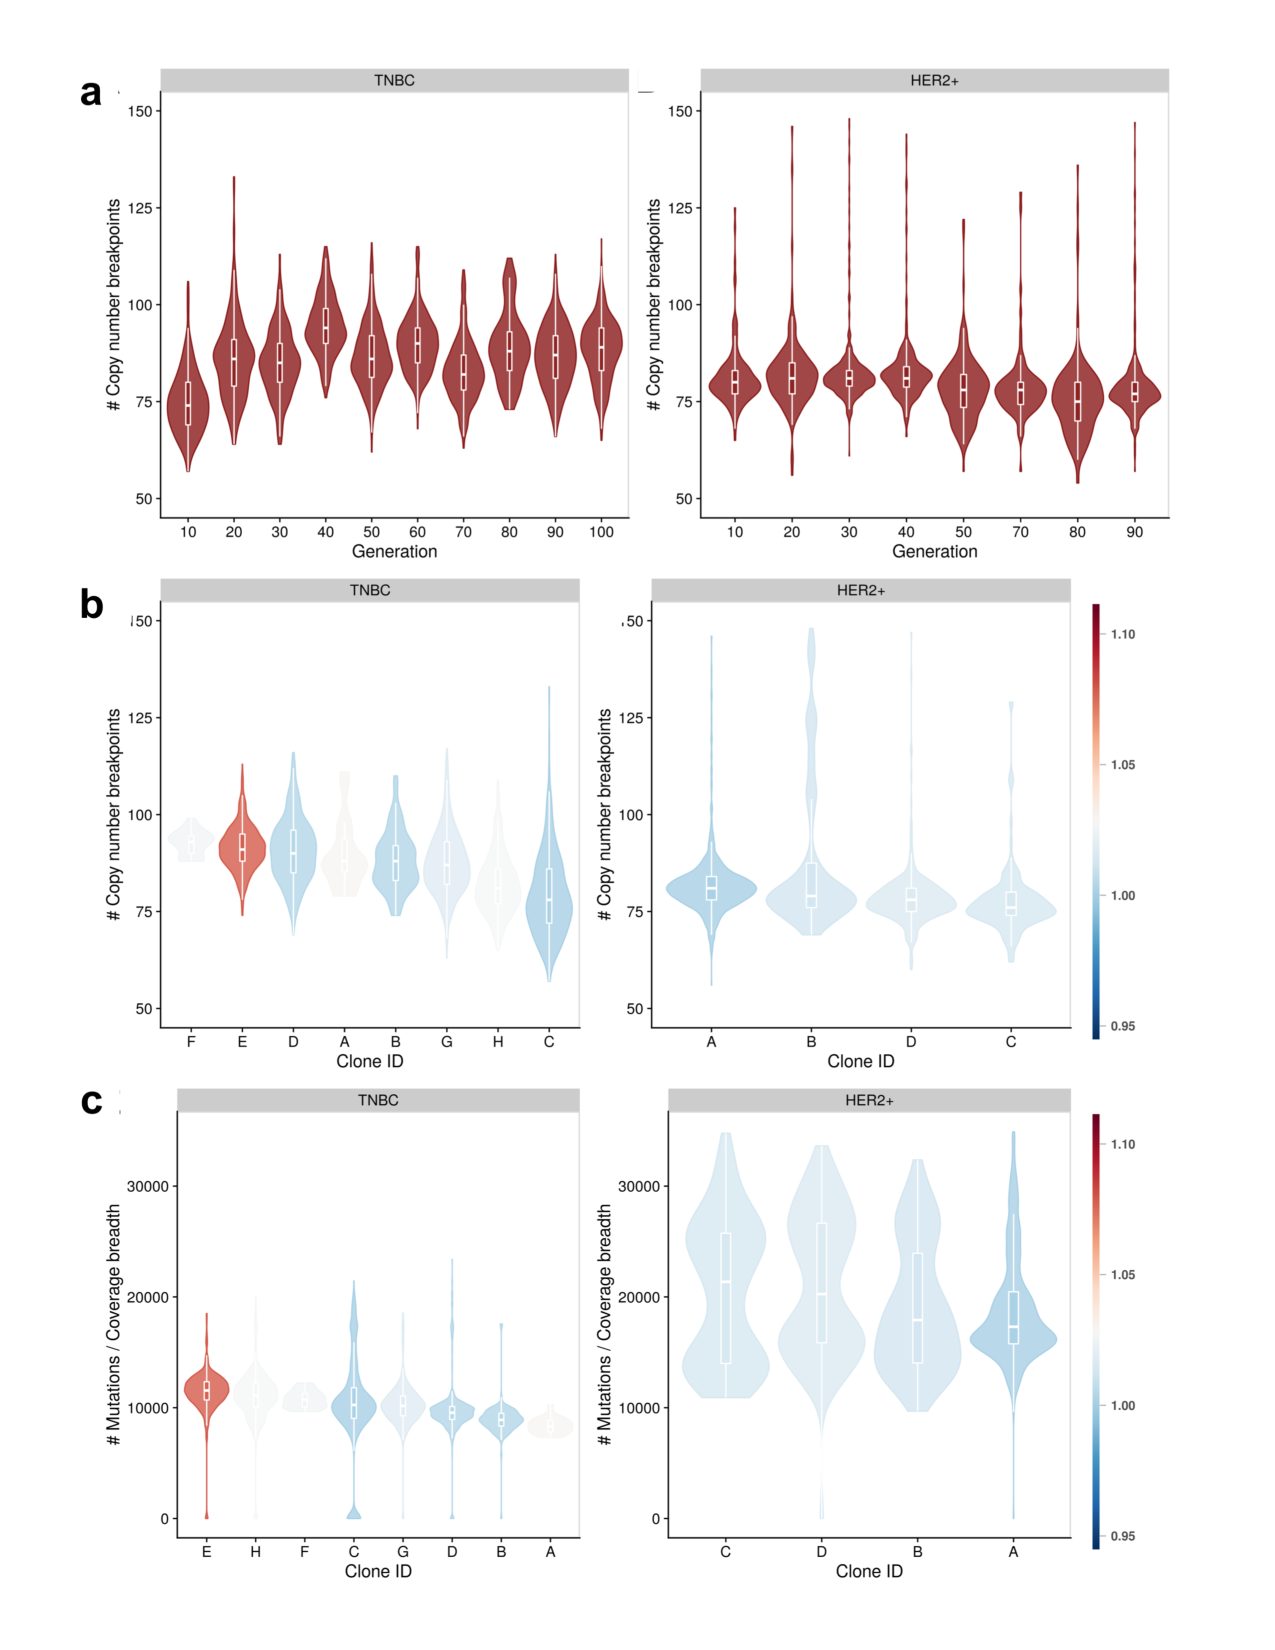
\includegraphics[width=\textwidth]{Figures/chap4/mutationanalysisbreakpoints.pdf}
  \caption[Structural variant and mutation rates of HER2+ and TNBC PDX]
	{\small
	\textbf{Structural variant and mutation rates of HER2+ and TNBC PDX.}
	    \textbf{(a)} Distribution over copy number
breakpoints/cell as a function of generation for left: TNBC, right: HER2+
   \textbf{(b)} Clone specific distributions over copy number breakpoints/cell, coloured by fitness coefficients for left: TNBC, right: HER2+
    \textbf{(c)} Clone specific distributions over point mutations/cell, coloured by fitness coefficients for left:TNBC, right:HER2+
}
    \label{fig:mutationanalysisbreakpoints}
    \end{figure}
%--------------------------------------------------------------------

\begin{figure}
\centering
  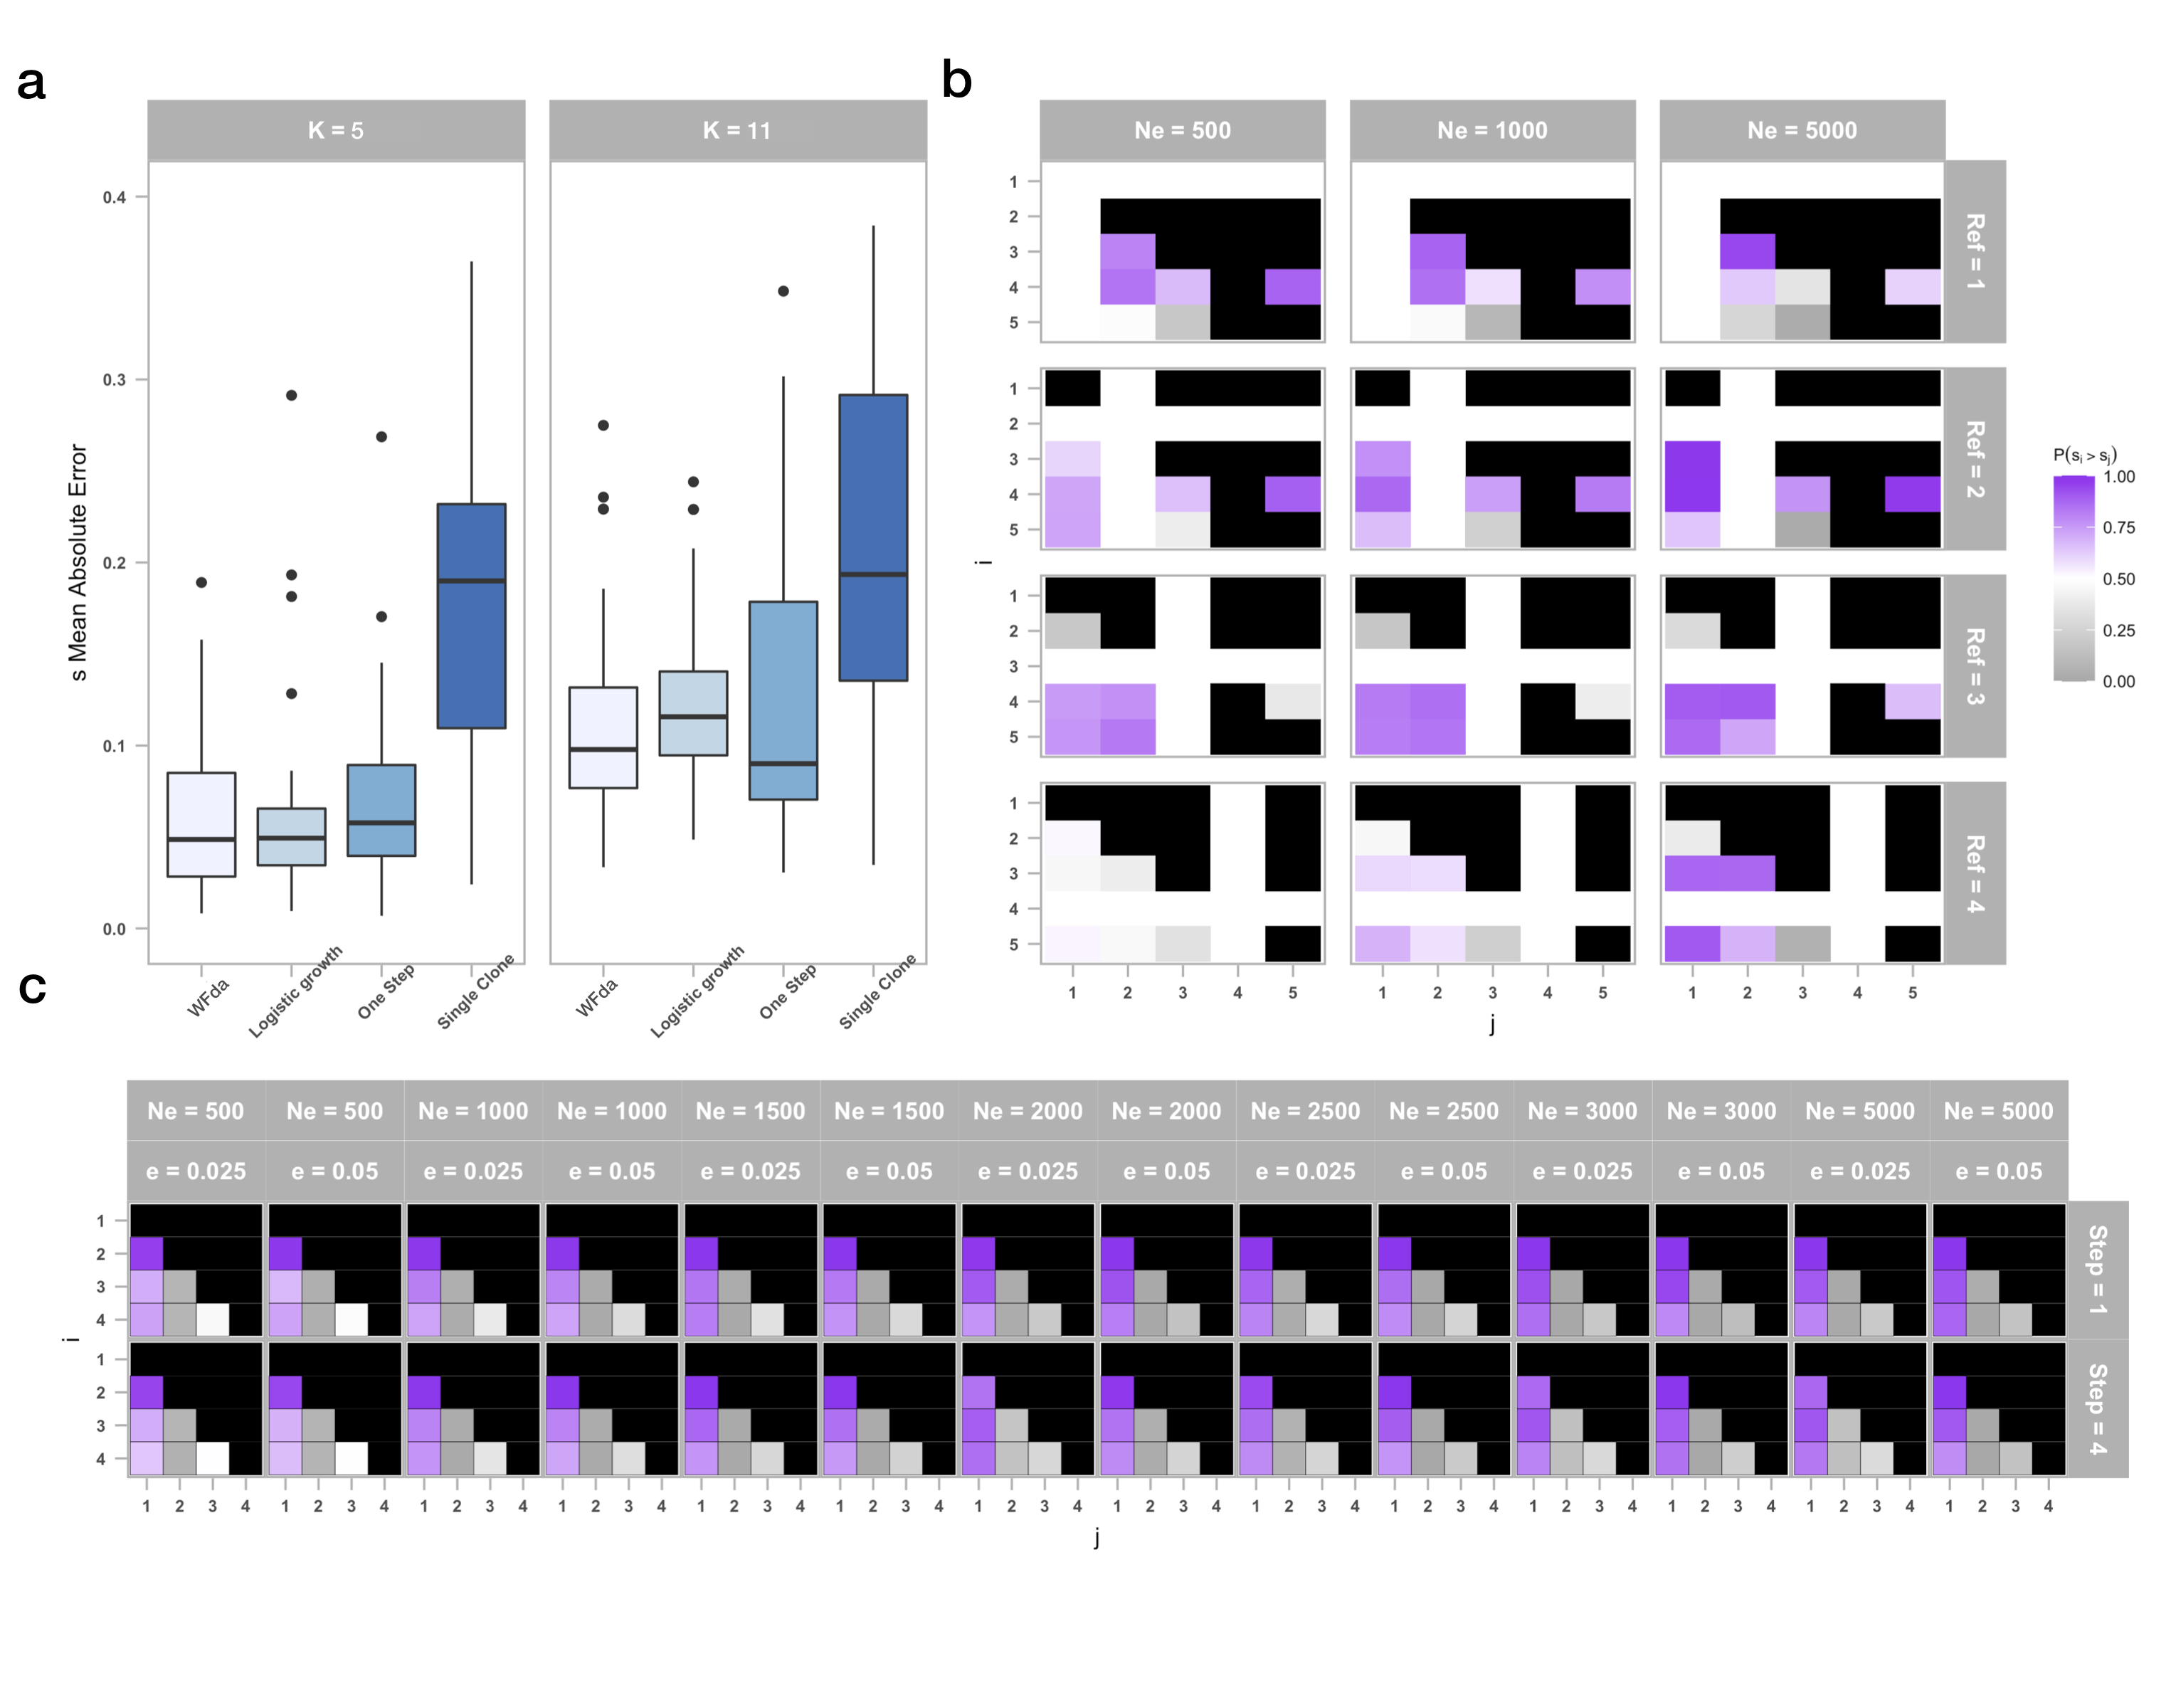
\includegraphics[width=\textwidth]{Figures/simulationspdx.png}
	
\caption[Simulation studies for the \texttt{fitClone} model]
	{\small
	\textbf{Simulation studies for the \texttt{fitClone} model.}
	  (a) Comparison to baseline methods for K = 5 clones (left) and K = 11 clones (right). (b) Posterior ordering of clones based on their inferred posterior selection coefficients across three values of effective population size (columns) and different choice of the reference clone (rows). (c) Posterior ordering of clones across different hyper parameters in the \texttt{fitClone} model. Effective population size in the range of 500 to 5,000 (top column), and observation error (bottom column). Minimum number of interpolations between two observations (rows).}
\label{fig:simulations}
\end{figure}


%-----------------------------------------------------------------


%---------------------------------------------------------------

\begin{figure}
\centering
  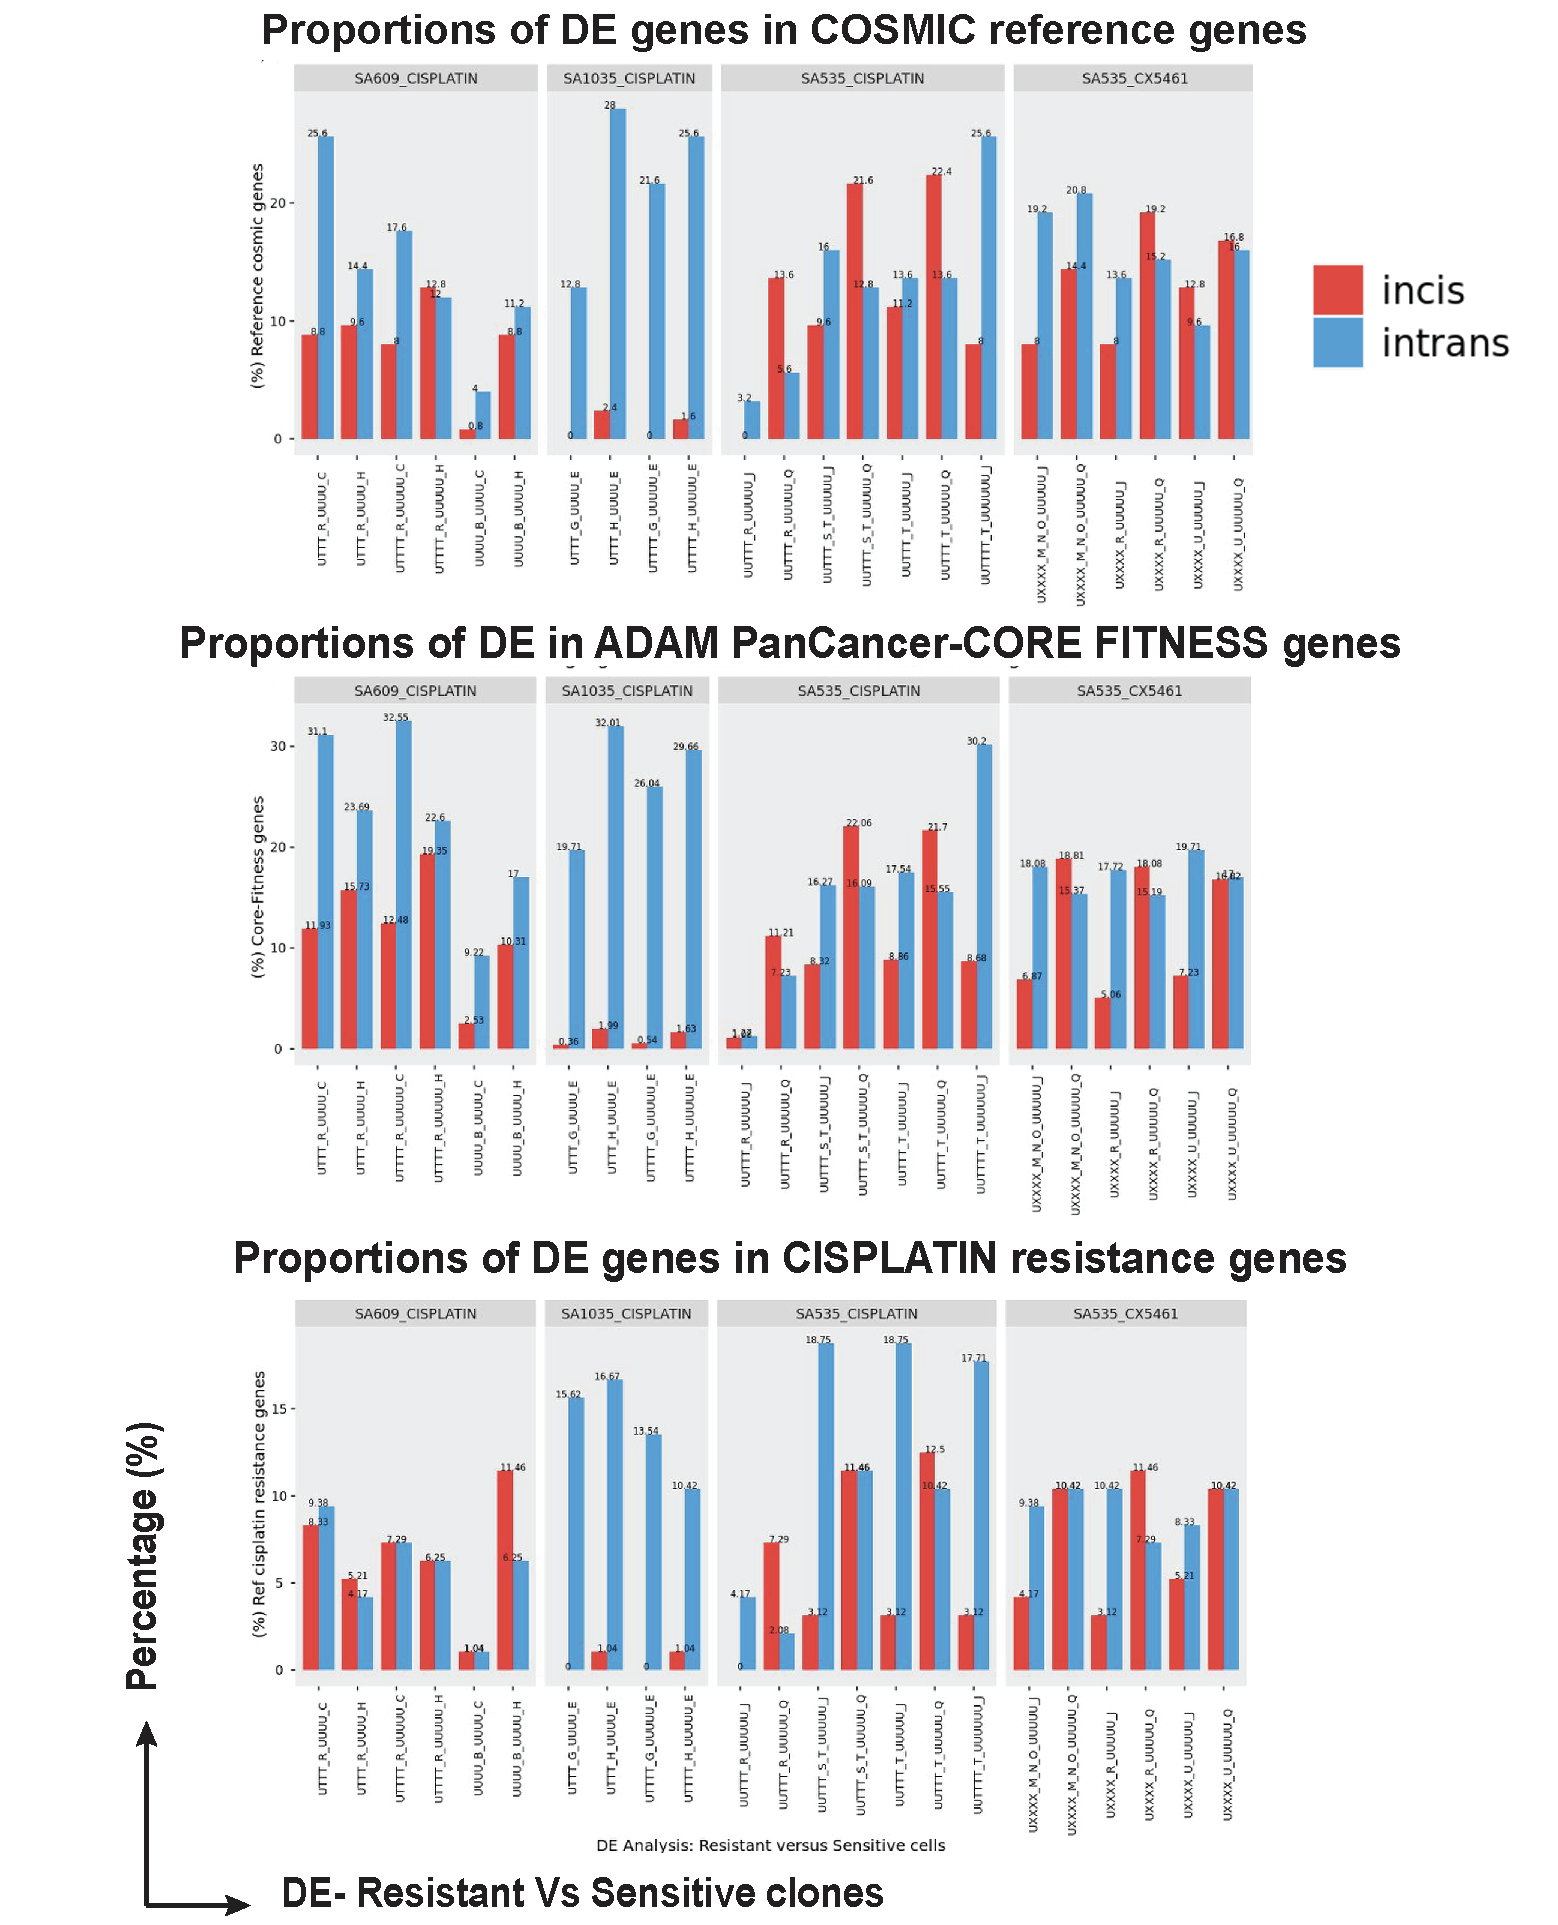
\includegraphics[width=\textwidth]{Figures/chap5/fig3_In_cispercentage.png}
	
\caption[Proportion of \textit{in cis} and \textit{in trans} regulated gene expression in scRNAseq data]
	{\small
	\textbf{Proportion of \textit{cis} and \textit{trans} regulated gene expression in scRNAseq data.}
	   Horizontal axis shows differential expression between two selected clones from all the three PDX treated and un-treated timeseries. Vertical axis gives percentage presence of genes \textit{in cis} or in trans. red bars represent in cis and blue bars represent in -trans regulated gene expression.
	   \textbf{(Upper)} This graph gives us percentage of genes by looking into the gene data set from COSMIC cancer gene dataset \cite{vogelstein2013cancer} that corresponds to our clone aware \ac{DE}.
	    \textbf{(Middle)} same like upper plot but looking into CORE FITNESS data set \cite{behan2019prioritization}.
	     \textbf{(Lower)} Same like above but looking into cisplatin related gene list curated from literature.
	    
	}
	\label{fig:fig3_In_cispercentage}
\end{figure}

%--------------------------------------------------------------------


\begin{figure}
\centering
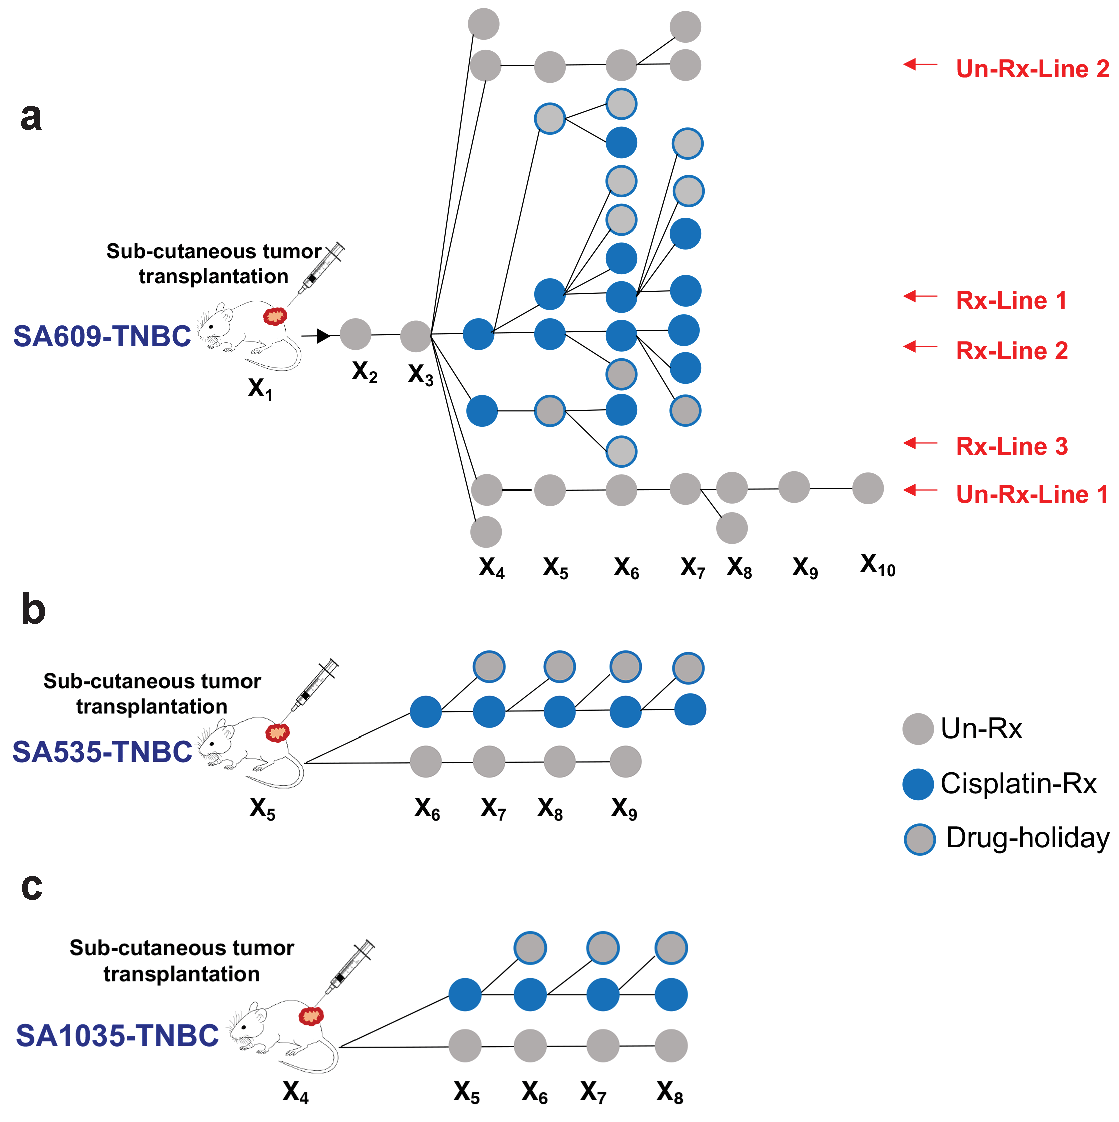
\includegraphics[width=\textwidth]{Figures/chap4/treatedtimeseriesmanuscript.pdf}
  \caption[TNBC PDX timeseries clonal dynamics under drug perturbations]
	{\small
	\textbf{TNBC PDX timeseries showing timepoint nodes sampled for single cell whole genome sequencing}
	     All nodes representing each PDX tumour were digested to acquire genomes of single cells (~200-600 cells/tumor). Extra replicate tumors at each time point are not shown in the diagram (n=2-4). Grey circles represent un-treated, blue represents Cisplatin treated and grey with blue outline presents drug-holiday samples 
	     \textbf{(a)} SA609-TNBC time series with replicates. DLP+ collected starting from X1 to X10 (Un-Rx line 1). Top grey branch indicating Un-Rx line 2. The middle three branches are cisplatin treated time series replicate branches 
	     \textbf{(b)} SA535-TNBC  showing the tumor nodes taken for DLP+ starting from X5 untreated  \textbf{(c)} SA1035-TNBC  showing the tumor nodes taken for DLP+ starting from X 4 untreated.}
     \label{fig:treatedtimeseriesmanuscript}

\end{figure}

%---------------------------------------------------------------------

 % Table generated by Excel2LaTeX from sheet 'Sheet1'
 \begin{table}[htbp]
   \centering
   \caption{Cisplatin related genes from last 10 years literature}
     \begin{tabular}{|l|l|l|l|r}
     
     \hline
     \multicolumn{4}{|l|}{Gene Names}  \\
     \hline
     
     VCAM1  & GCS    & BRCA2  & XAF1    \\
     VIM    & GST    & VDAC   & DYRK1B  \\
     SLC31A1 & MT     & BAX    & ERBB2 \\
     GST    & ERCC1  & BCL    & HSPs   \\
     HMGB   & MLH1   & BIRC5  & TMEM205 \\
     CTR1   & MSH2   & CPN    & PDGFR \\
     ATP7A  & POLH   & CASP   & IGF1R  \\
     ATP7B  & REV3   & MAPKs  & TRP14  \\
     MRP2   & REV7   & p63    & RAB7   \\
     GSH    & BRCA1  & TP53   & RAB8   \\
     \hline
     \end{tabular}%
   \label{tab:Cisplatinrelatedgenes}%
 \end{table}
%-------------------------------------------------------------------
\begin{figure}
\centering
  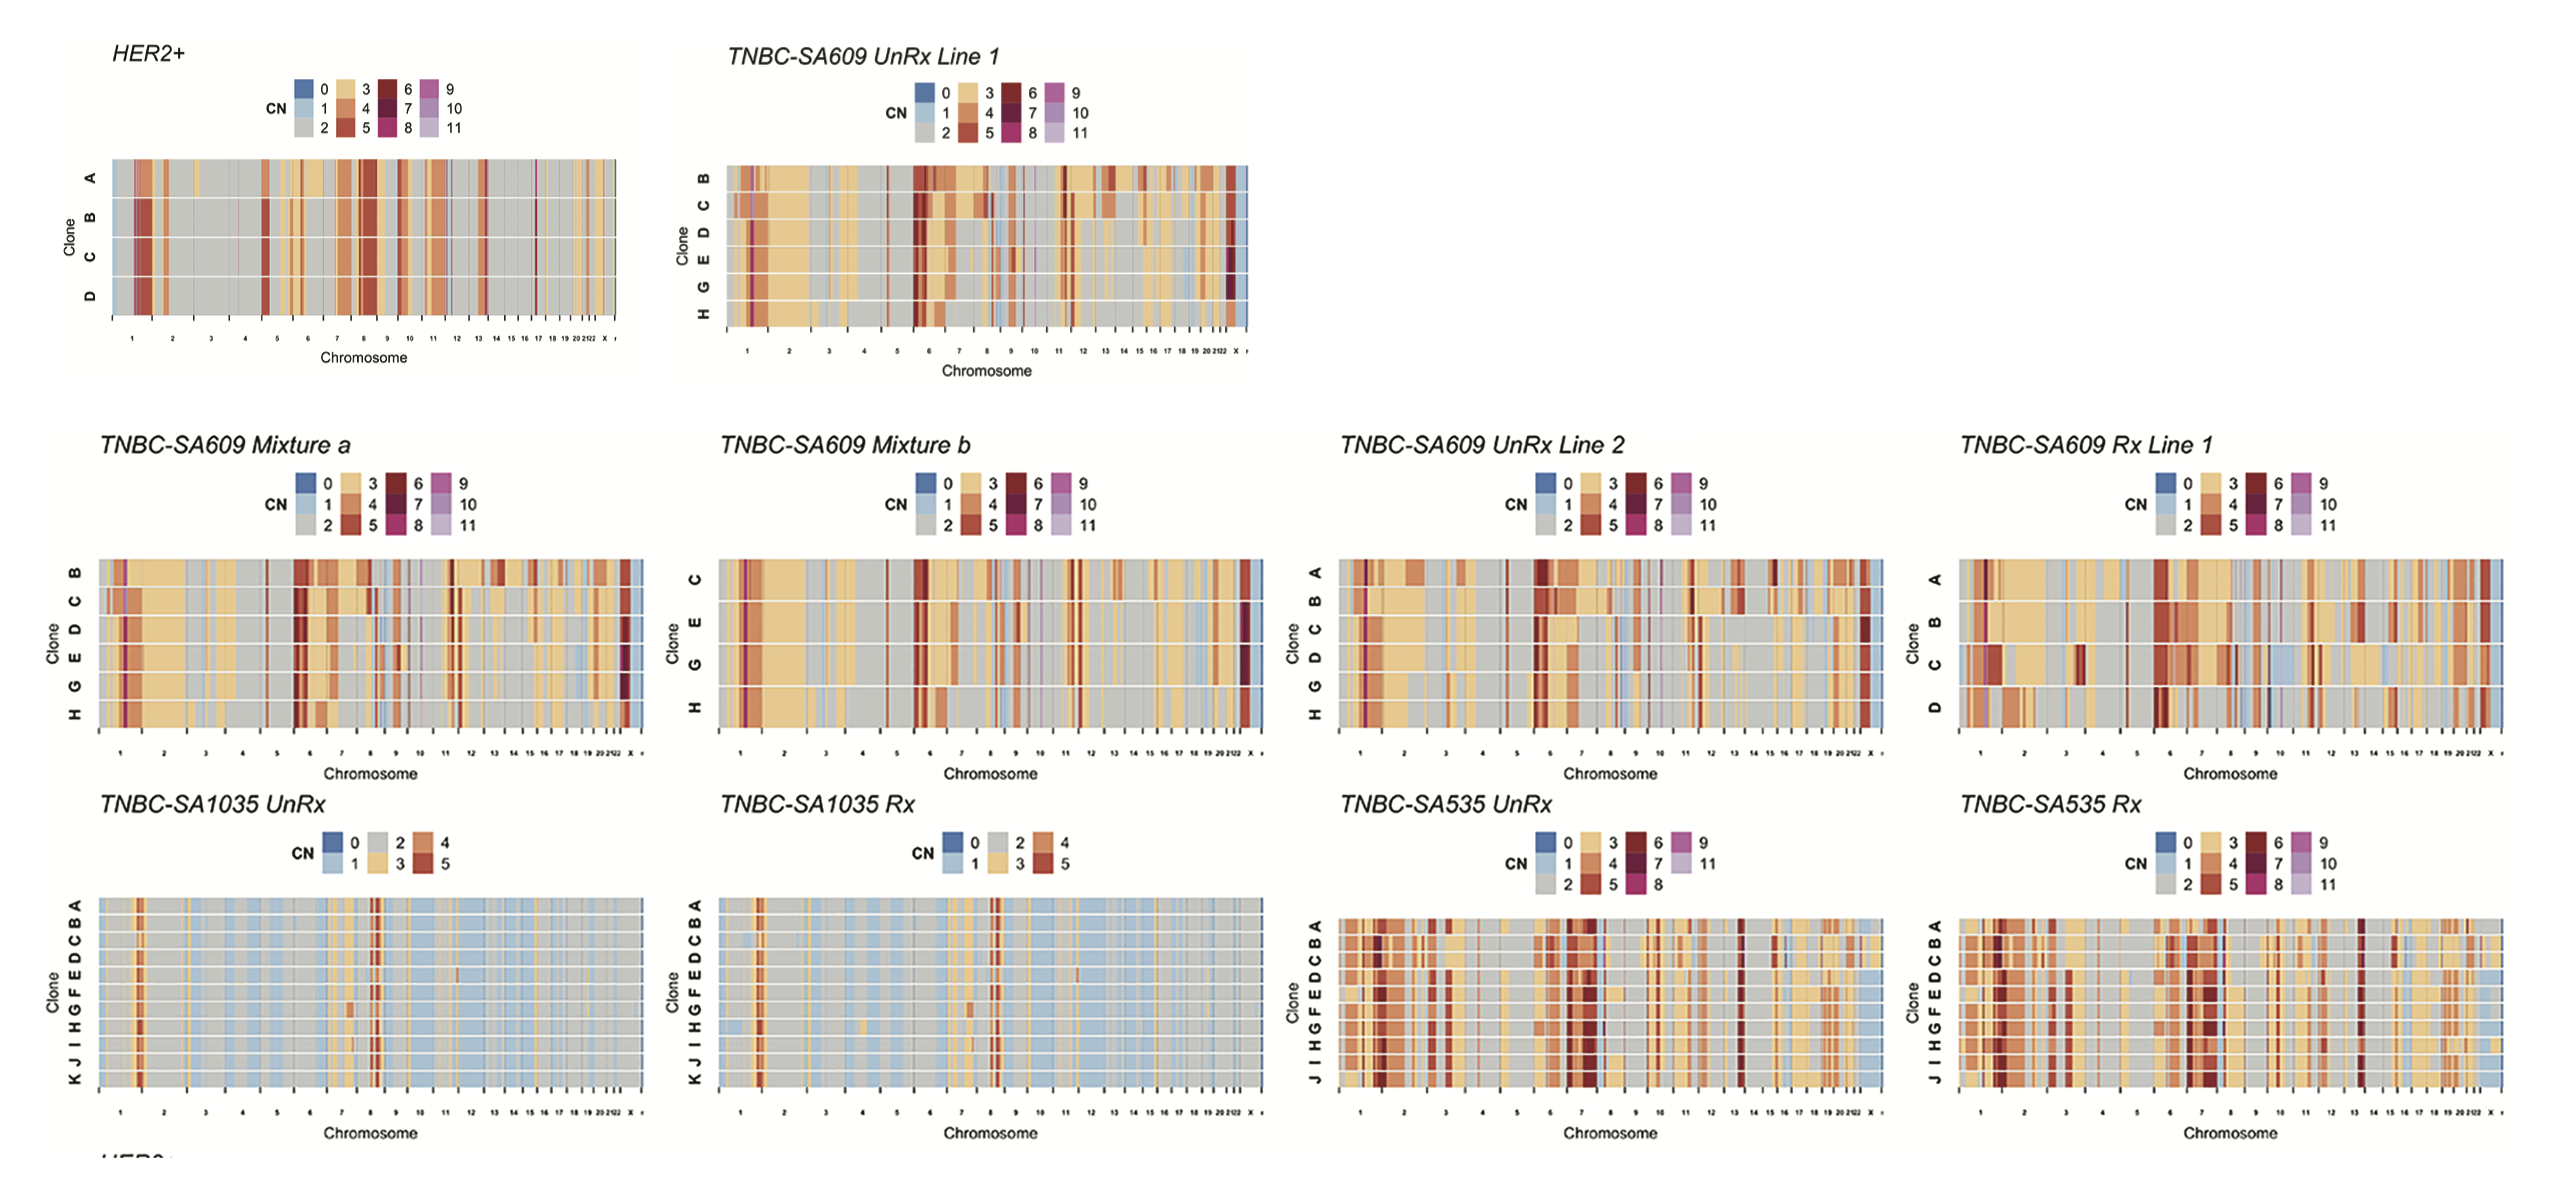
\includegraphics[width=\textwidth]{Figures/chap4/mediangenotypespdx.png}
\caption[Heatmaps of median genotypes]
	{\small
	\textbf{Heatmap representation of per clone median genotypes for TNBC PDX series SA609 UnRx Line 1 (U1), TNBC-SA609 mixtures a and b (Ma and Mb), SA609 UnRx Line 2 (U2), SA609 Rx line 1 (R1), SA1035 and SA535 treated and untreated (Un and Rx)}}.
	  
	 	\label{fig:mediangenotypes}
\end{figure} 


%-----------------------------------------------------------
\begin{figure}
\centering
  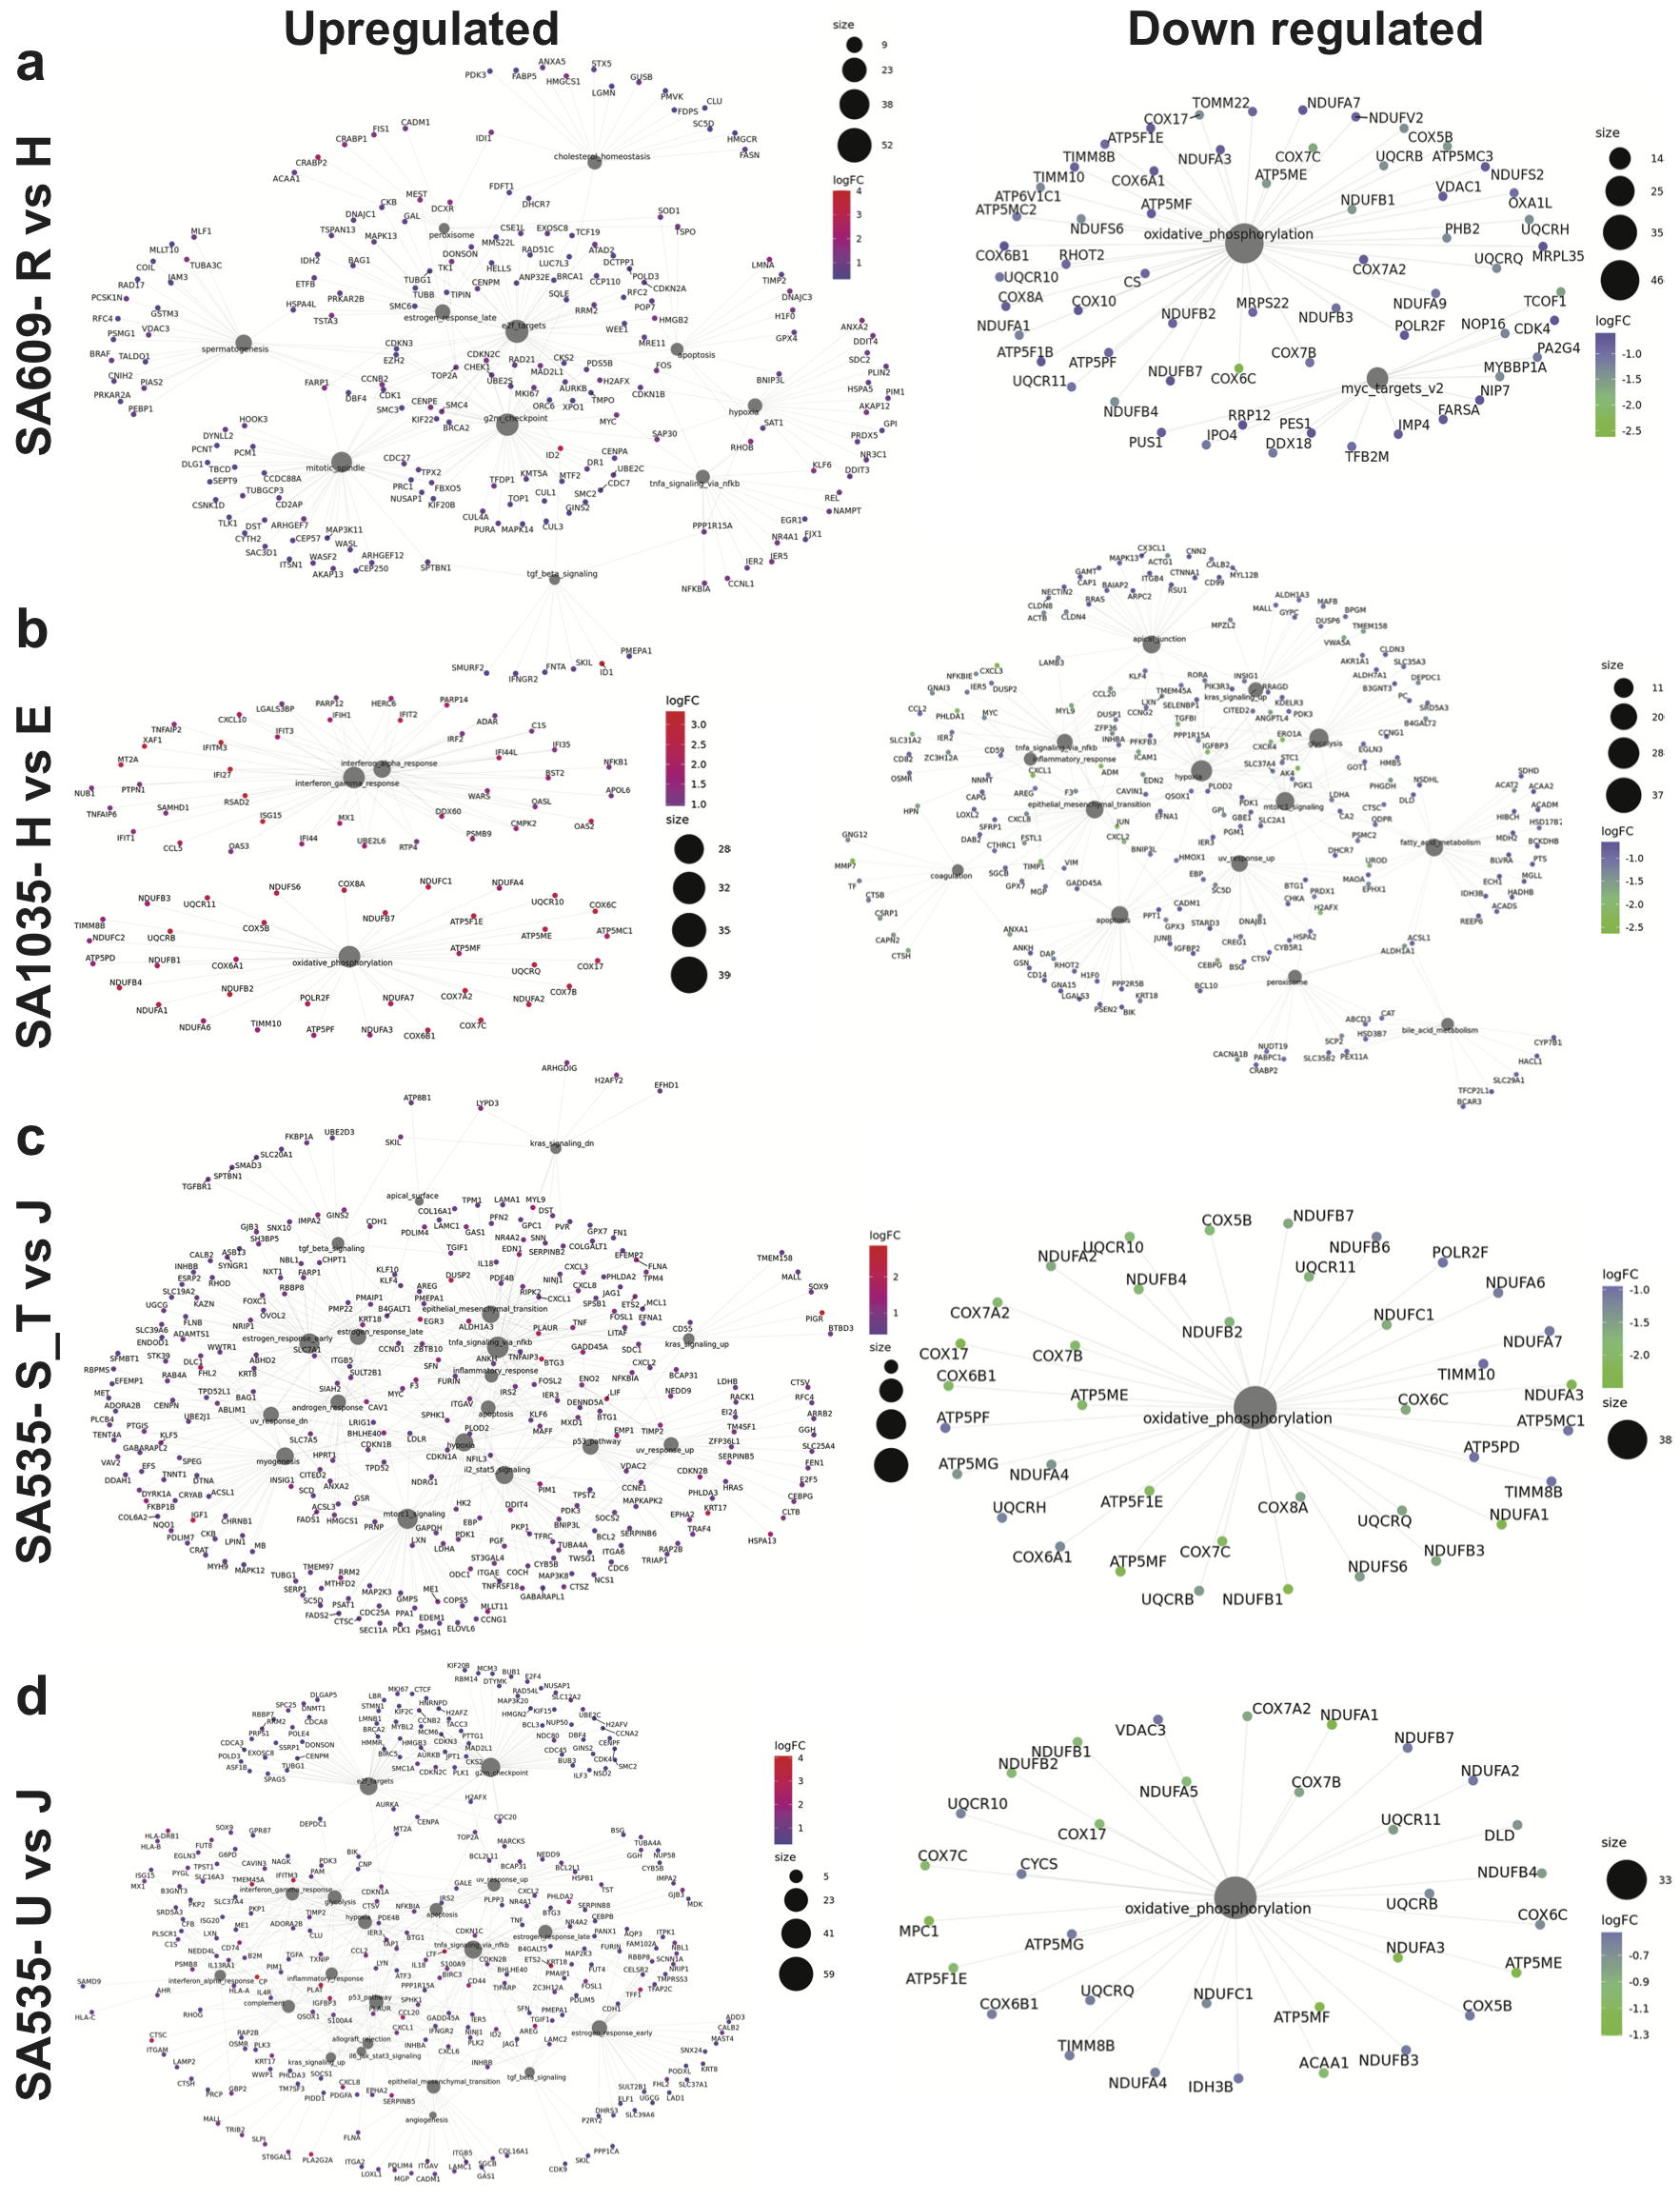
\includegraphics[width=\textwidth]{Figures/chap5/genenetworkanalysis.png}
\caption[DE of resistant and sensitive clonealign defined clones]
	{\small
	\textbf{Gene network analysis denoting connections denoting up-and-down regulated pathways across timeseries PDX}. Size of black circle indicates the number of genes, colour bars indicate the log fold change.
	\textbf{(a-d)} Genes in resistant vs sensitive clones of TNBCs-SASA609, SA1035, SA535 (cisplatin and CX-5461), respectively}
	  
	   	\label{fig:genenetworkanalysis}
\end{figure} 
%-----------------------------------------------------------

% Please add the following required packages to your document preamble:
% \usepackage{graphicx}
% \usepackage{lscape}
\begin{landscape}
\begin{table}[]
\caption{TNBC PDX-TMA scoring of IHC staining intensity}
\label{tab:TNBCTMAscoringIHC}
\resizebox{1.5\textwidth}{!}{%
\begin{tabular}{lllllllllllllllllllllll}
Timeseries & Timepoints & Treatment status & Block ID & ER  & ER \% & PR  & PR \% & HER 2  & HER 2 \% & Ki67  & Ki67 \% & EGFR  & EGFR \% & SMA  & SMA \% & CK8  & CK8 \% & CK14 & CK14 \% & CK5/6  & CK5/6 \% & E-cad \\
TNBC-SA609 & X4 & Un-Rx & 3080 & 0 & 0 & 0 & 0 & 0 & 0 & 3+ & 45 & 1+ & 50 & 0 & 0 & 0 & 0 & 0 & 0 & 0 & 0 & 0 \\
TNBC-SA609 & X5 & Un-Rx & 3223 & 0 & 0 & 0 & 0 & 0 & 0 & 3+ & 50 & 1+ & 40 & 0 & 0 & 0 & 0 & 0 & 0 & 0 & 0 & 0 \\
TNBC-SA609 & X6 & Un-Rx & 3447 & 0 & 0 & 0 & 0 & 0 & 0 & 3+ & 45 & 2+ & 30 & 3+ & 0-1 & 0 & 0 & 0 & 0 & 0 & 0 & 0 \\
TNBC-SA609 & X4 & Rx & 3083 & 0 & 0 & 0 & 0 & 0 & 0 & 3+ & 60 & 1+ & 60 & 0 & 0 & 0 & 0 & 0 & 0 & 0 & 0 & 0 \\
TNBC-SA609 & X4 & Rx & 3084 & 0 & 0 & 0 & 0 & 0 & 0 & 3+ & 70 & 1+ & 70 & 0 & 0 & 0 & 0 & 0 & 0 & 0 & 0 & 0 \\
TNBC-SA609 & X5 & Rx & 3230 & 0 & 0 & 0 & 0 & 0 & 0 & 3+ & 45 & 1+ & 50 & 0 & 0 & 0 & 0 & 0 & 0 & 0 & 0 & 0 \\
TNBC-SA609 & X5 & dh & 3231 & 0 & 0 & 0 & 0 & 0 & 0 & 3+ & 35 & 1+ & 75 & 0 & 0 & 0 & 0 & 0 & 0 & 0 & 0 & 0 \\
TNBC-SA609 & X5 & Rx-recur & 3235 & 0 & 0 & 0 & 0 & 0 & 0 & 3+ & 35 & 2+ & 50 & 0 & 0 & 0 & 0 & 0 & 0 & 0 & 0 & 0 \\
TNBC-SA609 & X6 & Rx & 3400 & 0 & 0 & 0 & 0 & 0 & 0 & 3+ & 35 & 1+ & 40 & 0 & 0 & 0 & 0 & 0 & 0 & 0 & 0 & 0 \\
TNBC-SA609 & X6 & dh & 3401 & 0 & 0 & 0 & 0 & 0 & 0 & 3+ & 30 & 1+ & 10 & 0 & 0 & 0 & 0 & 0 & 0 & 0 & 0 & 0 \\
TNBC-SA609 & X6 & Rx & 3404 & 0 & 0 & 0 & 0 & 0 & 0 & 3+ & 35 & 1+ & 40 & 0 & 0 & 0 & 0 & 0 & 0 & 0 & 0 & 0 \\
TNBC-SA609 & X7 & Rx & 3505 & 0 & 0 & 0 & 0 & 0 & 0 & 3+ & 50 & 1+ & 40 & 0 & 0 & 0 & 0 & 0 & 0 & 0 & 0 & 0 \\
TNBC-SA609 & X7 & Rx & 3506 & 0 & 0 & 1+ & 0-1 & 0 & 0 & 3+ & 60 & 1+ & 60 & 0 & 0 & 0 & 0 & 0 & 0 & 0 & 0 & 0 \\
TNBC-SA609 & X7 & dh & 3510 & 0 & 0 & 1+ & 0-1 & 0 & 0 & 3+ & 45 & 1+ & 40 & 0 & 0 & 0 & 0 & 0 & 0 & 0 & 0 & 0 \\
TNBC-SA609 & X5 & Rx & 3226 & 0 & 0 & 0 & 0 & 0 & 0 & 3+ & 45 & 1+ & 35 & 0 & 0 & 0 & 0 & 0 & 0 & 0 & 0 & 0 \\
TNBC-SA609 & X6 & Rx & 3387 & 0 & 0 & 0 & 0 & 0 & 0 & 3+ & 50 & 1+ & 50 & 0 & 0 & 0 & 0 & 0 & 0 & 0 & 0 & 0 \\
TNBC-SA609 & X7 & Rx & 3573 & 0 & 0 & 0 & 0 & 0 & 0 & 3+ & 90 & 3+ & 5 & 0 & 0 & 0 & 0 & 0 & 0 & 0 & 0 & 0 \\
TNBC-SA609 & X7 & Rx & 3578 & 0 & 0 & 0 & 0 & 0 & 0 & 3+ & 90 & 1+ & 10 & 0 & 0 & 0 & 0 & 0 & 0 & 0 & 0 & 0 \\
TNBC-SA609 & X7 & dh & 3508 & 0 & 0 & 0 & 0 & 0 & 0 & 3+ & 35 & 1+ & 35 & 0 & 0 & 0 & 0 & 0 & 0 & 0 & 0 & 0 \\
TNBC-SA609 & X7 & dh & 3577 & 0 & 0 & 0 & 0 & 0 & 0 & 3+ & 80 & 1+ & 05-Jan & 0 & 0 & 0 & 0 & 0 & 0 & 0 & 0 & 0 \\
 &  &  &  &  &  &  &  &  &  &  &  &  &  &  &  &  &  &  &  &  &  &  \\
TNBC-SA1035 & X4 & Un-Rx & 2879 & 1+ & 0-1 & 0 & 0 & 0 & 0 & 3+ & 65 & 3+ & 100 & 0 & 0 & 1+ & 25 & 3+ & 10 & 2+ & 10 & 3+ \\
TNBC-SA1035 & X5 & Un-Rx & 3021 & 1+ & 0-1 & 0 & 0 & 0 & 0 & 3+ & 50 & 3+ & 100 & 0 & 0 & 1+ & 5 & 3+ &  & 2+ & 10 & 3+ \\
TNBC-SA1035 & X6 & Un-Rx & 3216 & 1+ & 0-1 & 0 & 0 & 0 & 0 & 2+ & 65 & 3+ & 100 & 0 & 0 & 2+ & 5 & 3+ & 0-1 & 2+ & 0-1 & 3+ \\
TNBC-SA1035 & X7 & Un-Rx & 3502 & 1+ & 0-1 & 0 & 0 & 0 & 0 & 3+ & 70 & 3+ & 100 & 0 & 0 & 1+ & 5 & 3+ & 5 & 2+ & 10 & 3+ \\
TNBC-SA1035 & X8 & Un-Rx & 3631 & 1+ & 0-1 & 0 & 0 & 0 & 0 & 3+ & 80 & 3+ & 100 & 0 & 0 & 1+ & 0-1 & 3+ & 0-1 & 2+ & 1 & 3+ \\
TNBC-SA1035 & X5 & Rx & 3015 & 1+ & 0-1 & 0 & 0 & 0 & 0 & 3+ & 50 & 3+ & 95 & 0 & 0 & 2+ & 70 & 3+ & 10 & 3+ & 40 & 3+ \\
TNBC-SA1035 & X6 & dh & 3209 & 1+ & 0-1 & 0 & 0 & 0 & 0 & 3+ & 60 & 3+ & 100 & 0 & 0 & 2+ & 5 & 3+ & 1 & 2+ & 10 & 3+ \\
TNBC-SA1035 & X6 & Rx & 3211 & 1+ & 0-1 & 0 & 0 & 0 & 0 & 3+ & 50 & 3+ & 100 & 0 & 0 & 2+ & 20 & 3+ & 1 & 2+ & 30 & 3+ \\
TNBC-SA1035 & X7 & Rx & 3338 & 1+ & 0-1 & 0 & 0 & 0 & 0 & 3+ & 80 & 3+ & 100 & 0 & 0 & 1+ & 5 & 3+ & 5-10 & 2+ & 15 & 3+ \\
TNBC-SA1035 & X7 & dh & 3340 & 1+ & 0-1 & 0 & 0 & 0 & 0 & 3+ & 60 & 3+ & 100 & 0 & 0 & 2+ & 5 & 3+ & 1 & 2+ & 10 & 3+ \\
TNBC-SA1035 & X8 & Rx & 3425 & 1+ & 0-1 & 0 & 0 & 0 & 0 & 3+ & 70 & 3+ & 100 & 0 & 0 & 1+ & 5 & 3+ & 1 & 2+ & 5 & 3+ \\
 &  &  &  &  &  &  &  &  &  &  &  &  &  &  &  &  &  &  &  &  &  &  \\
TNBC-SA535 & X6 & Un-Rx & 3099 & 0 & 0 & 0 & 0 & 0 & 0 & 3+ & 25 & 3+ & 90 & 0 & 0 & 2+ & 65 & 0 & 0 & 2+ & 5-10 & 3+ \\
TNBC-SA535 & X7 & Un-Rx & 3448 & 0 & 0 & 0 & 0 & 0 & 0 & 3+ & 30 & 3+ & 100 & 0 & 0 & 2+ & 15 & 0 & 0 & 2+ & 0-1 & 3+ \\
TNBC-SA535 & X6 & Rx & 3101 & 1+ & 0-1 & 0 & 0 & 0 & 0 & 3+ & 35 & 2+ & 95 & 0 & 0 & 2+ & 80 & 3+ & 1 & 2+ & 5 & 3+ \\
TNBC-SA535 & X7 & Rx-cis & 3304 & 0 & 0 & 0 & 0 & 0 & 0 & 3+ & 35 & 2+ & 80 & 0 & 0 & 2+ & 95 & 3+ & 0-1 & 2+ & 1 & 3+ \\
TNBC-SA535 & X7 & dh-cis & 3305 & 0 & 0 & 0 & 0 & 0 & 0 & 3+ & 35 & 2+ & 90 & 0 & 0 & 3+ & 95 & 3+ & 1 & 2+ & 5 & 3+ \\
TNBC-SA535 & X8 & Rx-cis & 3431 & 1+ & 0-1 & 0 & 0 & 0 & 0 & 3+ & 45 & 2+ & 95 & 0 & 0 & 2+ & 95 & 3+ & 0-1 & 2+ & 5 & 3+ \\
TNBC-SA535 & X8 & dh-cis & 3434 & 1+ & 1 & 0 & 0 & 0 & 0 & 3+ & 35 & 2+ & 85 & 0 & 0 & 2+ & 95 & 3+ & 1 & 2+ & 10 & 3+ \\
TNBC-SA535 & X9 & dh-cis & 3616 & 1+ & 1 & 0 & 0 & 0 & 0 & 3+ & 40 & 2+ & 95 & 0 & 0 & 2+ & 75 & 0 & 0 & 2+ & 10 & 3+ \\
TNBC-SA535 & X9 & Rx-cis & 3617 & 1+ & 1 & 0 & 0 & 0 & 0 & 3+ & 45 & 2+ & 90 & 0 & 0 & 2+ & 90 & 3+ & 1 & 2+ & 5 & 3+
\end{tabular}%
}
\end{table}
\end{landscape} 
%-------------------------------------------------------------------
%-------------------------------------------------------------

 % Table generated by Excel2LaTeX from sheet 'Sheet1'
 \begin{table}[htbp]
   \centering
   \caption{TNBC-SA609-Upregulated top genes in clusters}
     \begin{tabular}{|l|l|l|}
     \hline
     Genes in SA609 & Cluster & Gene\_regulation \\
     \hline
     ARF5 & blue & In\_cis\_Increase\_UpRegulated \\
     POLR2I & blue & In\_cis\_Increase\_UpRegulated \\
     DSCR8 & blue & In\_cis\_Increase\_UpRegulated \\
     DRAP1 & blue & In\_cis\_Increase\_UpRegulated \\
     SCAND1 & blue & In\_cis\_Increase\_UpRegulated \\
     PCSK1N & blue & In\_trans\_UpRegulated \\
     GAGE2A & blue & In\_trans\_UpRegulated \\
     VCX & blue & In\_trans\_UpRegulated \\
     C19orf24 & blue & In\_trans\_UpRegulated \\
     TSPO & blue & In\_trans\_UpRegulated \\
     NUDT3 & turquoise & In\_cis\_Increase\_UpRegulated \\
     PPDPF & turquoise & In\_cis\_Increase\_UpRegulated \\
     KMT2B & turquoise & In\_cis\_Increase\_UpRegulated \\
     POM121 & turquoise & In\_cis\_Increase\_UpRegulated \\
     TCF4 & turquoise & In\_cis\_Increase\_UpRegulated \\
     H3F3B & turquoise & In\_trans\_UpRegulated \\
     FAAP20 & turquoise & In\_trans\_UpRegulated \\
     FAM207A & turquoise & In\_trans\_UpRegulated \\
     ZFHX3 & turquoise & In\_trans\_UpRegulated \\
     PITX1 & turquoise & In\_trans\_UpRegulated \\
     HSPA1A & brown & In\_cis\_Increase\_UpRegulated \\
     CYR61 & brown & In\_cis\_Increase\_UpRegulated \\
     ID1 & brown & In\_cis\_Increase\_UpRegulated \\
     EIF3H & brown & In\_cis\_Increase\_UpRegulated \\
     OSTC & brown & In\_cis\_Increase\_UpRegulated \\
     EIF4A2 & brown & In\_trans\_UpRegulated \\
     FOS & brown & In\_trans\_UpRegulated \\
     RHOB & brown & In\_trans\_UpRegulated \\
     SQLE & brown & In\_trans\_UpRegulated \\
     CCNL1 & brown & In\_trans\_UpRegulated \\
     \hline
     \end{tabular}%
   \label{tab:SA609upregulatedgenesinclusters}%
 \end{table}%
%-------------------------------------------------------------
 
  % Table generated by Excel2LaTeX from sheet 'SA609downregulatedtopgenesclust'
 \begin{table}[htbp]
   \centering
   \caption{TNBC-SA609-downregulated top genes in clusters}
     \begin{tabular}{|l|l|l|r}
     \hline
     Genes in SA609 & Cluster & Gene\_Regulation   \\
     \hline
     CDK4 & yellow & In\_cis\_Decrease\_DownRegulated   \\
     PPIF & yellow & In\_cis\_Decrease\_DownRegulated   \\
     H2AFJ & yellow & In\_cis\_Decrease\_DownRegulated  \\
     MGST1 & yellow & In\_cis\_Decrease\_DownRegulated   \\
     LEPROT & yellow & In\_cis\_Decrease\_DownRegulated   \\
     PAICS & yellow & In\_trans\_DownRegulated   \\
     NCS1 & yellow & In\_trans\_DownRegulated   \\
     SAMD1 & yellow & In\_trans\_DownRegulated   \\
     JPT1 & yellow & In\_trans\_DownRegulated   \\
     NUP88 & yellow & In\_trans\_DownRegulated   \\
     TPT1 & blue & In\_cis\_Decrease\_DownRegulated   \\
     COX6C & blue & In\_cis\_Decrease\_DownRegulated   \\
     EIF3E & blue & In\_cis\_Decrease\_DownRegulated   \\
     EIF4B & blue & In\_cis\_Decrease\_DownRegulated  \\
     PABPC1 & blue & In\_cis\_Decrease\_DownRegulated   \\
     RBM3 & blue & In\_trans\_DownRegulated   \\
     RACK1 & blue & In\_trans\_DownRegulated   \\
     UQCRH & blue & In\_trans\_DownRegulated   \\
     LDHB & blue & In\_trans\_DownRegulated   \\
     SSR2 & blue & In\_trans\_DownRegulated   \\
     PCBP2 & green & In\_cis\_Decrease\_DownRegulated   \\
     DGCR6L & green & In\_cis\_Decrease\_DownRegulated   \\
     ZBED1 & green & In\_cis\_Decrease\_DownRegulated   \\
     JMJD4 & green & In\_cis\_Decrease\_DownRegulated   \\
     MRPL28 & green & In\_cis\_Decrease\_DownRegulated   \\
     CDK2AP1 & green & In\_trans\_DownRegulated   \\
     GIGYF2 & green & In\_trans\_DownRegulated   \\
     PSMD1 & green & In\_trans\_DownRegulated   \\
     MFAP2 & green & In\_trans\_DownRegulated   \\
     PES1 & green & In\_trans\_DownRegulated   \\
     \hline
     \end{tabular}%
   \label{tab:SA609downrregulatedgenesinclusters}%
 \end{table}%
 %----------------------------------------------------------------
 
  % Table generated by Excel2LaTeX from sheet 'SA1035upregulatedtopgenescluste'
 \begin{table}[htbp]
   \centering
   \caption{TNBC-SA1035-Upregulated top genes in clusters}
     \begin{tabular}{|l|l|l|r}
        \hline
     Gene ID & Cluster & Gene\_Regulation   \\
        \hline
     SIVA1 & yellow & In\_cis\_Increase\_UpRegulated   \\
     AKT1 & yellow & In\_cis\_Increase\_UpRegulated   \\
     CLMN & yellow & In\_cis\_Increase\_UpRegulated  \\
     DYNC1H1 & yellow & In\_cis\_Increase\_UpRegulated   \\
     GLRX5 & yellow & In\_cis\_Increase\_UpRegulated   \\
     PCBP2 & yellow & In\_trans\_UpRegulated   \\
     ATP6V1F & yellow & In\_trans\_UpRegulated   \\
     BCL7C & yellow & In\_trans\_UpRegulated   \\
     TPM2 & yellow & In\_trans\_UpRegulated   \\
     FAM96B & yellow & In\_trans\_UpRegulated   \\
     COX6C & green & In\_cis\_Increase\_UpRegulated   \\
     ATP5MPL & green & In\_cis\_Increase\_UpRegulated   \\
     MRPL33 & green & In\_cis\_Increase\_UpRegulated   \\
     PCMTD1 & green & In\_cis\_Increase\_UpRegulated   \\
     NBN & green & In\_cis\_Increase\_UpRegulated   \\
     OST4 & green & In\_trans\_UpRegulated   \\
     TOMM7 & green & In\_trans\_UpRegulated   \\
     FMC1 & green & In\_trans\_UpRegulated   \\
     COX7A2 & green & In\_trans\_UpRegulated   \\
     MGST3 & green & In\_trans\_UpRegulated   \\
     ENY2 & blue & In\_cis\_Increase\_UpRegulated   \\
     POLR2K & blue & In\_cis\_Increase\_UpRegulated   \\
     PRKDC & blue & In\_cis\_Increase\_UpRegulated   \\
     TCEA1 & blue & In\_cis\_Increase\_UpRegulated   \\
     DESI2 & blue & In\_cis\_Increase\_UpRegulated   \\
     HSPE1 & blue & In\_trans\_UpRegulated   \\
     LRPPRC & blue & In\_trans\_UpRegulated   \\
     RRP15 & blue & In\_trans\_UpRegulated   \\
     NDUFB3 & blue & In\_trans\_UpRegulated   \\
     ITGAE & blue & In\_trans\_UpRegulated   \\
     \hline
     \end{tabular}%
   \label{tab:SA1035upregulatedgenesinclusters}%
 \end{table}%
%------------------------------------------------

 % Table generated by Excel2LaTeX from sheet 'Sheet1'
 \begin{table}[htbp]
   \centering
   \caption{SA1035-downregulated top genes in clusters}
     \begin{tabular}{|l|l|l|r}
     \hline
     Gene ID & Cluster & Gene\_Regulation   \\
     \hline
     FXYD5 & turquoise & In\_cis\_Decrease\_DownRegulated  \\
     TMEM147 & turquoise & In\_cis\_Decrease\_DownRegulated  \\
     CRYAB & turquoise & In\_cis\_Decrease\_DownRegulated  \\
     BARX2 & turquoise & In\_cis\_Decrease\_DownRegulated   \\
     SC5D & turquoise & In\_cis\_Decrease\_DownRegulated   \\
     ARPC1B & turquoise & In\_trans\_DownRegulated   \\
     TMEM79 & turquoise & In\_trans\_DownRegulated   \\
     RHOC & turquoise & In\_trans\_DownRegulated   \\
     PRSS22 & turquoise & In\_trans\_DownRegulated   \\
     TACSTD2 & turquoise & In\_trans\_DownRegulated   \\
     ATP6V0B & blue & In\_cis\_Decrease\_DownRegulated   \\
     H2AFX & blue & In\_cis\_Decrease\_DownRegulated  \\
     UQCRFS1 & blue & In\_cis\_Decrease\_DownRegulated  \\
     ZNF302 & blue & In\_cis\_Decrease\_DownRegulated   \\
     BCAS2 & blue & In\_cis\_Decrease\_DownRegulated   \\
     PRDX1 & blue & In\_trans\_DownRegulated   \\
     HNRNPA1 & blue & In\_trans\_DownRegulated   \\
     MYL12B & blue & In\_trans\_DownRegulated   \\
     MFGE8 & blue & In\_trans\_DownRegulated   \\
     ATP5PB & blue & In\_trans\_DownRegulated   \\
     LRP3 & green & In\_cis\_Decrease\_DownRegulated   \\
     PLEKHF1 & green & In\_cis\_Decrease\_DownRegulated   \\
     GPI & green & In\_cis\_Decrease\_DownRegulated  \\
     MPZL2 & green & In\_cis\_Decrease\_DownRegulated  \\
     C11orf1 & green & In\_cis\_Decrease\_DownRegulated   \\
     HSPA1A & green & In\_trans\_DownRegulated  \\
     ACTB & green & In\_trans\_DownRegulated  \\
     DNAJB1 & green & In\_trans\_DownRegulated   \\
     JUN & green & In\_trans\_DownRegulated   \\
     ARHGAP26 & green & In\_trans\_DownRegulated  \\
       \hline
     \end{tabular}%
   \label{tab:SA1035downregulatedgenesinclusters}%
 \end{table}%
%--------------------------------------------------------------------

 % Table generated by Excel2LaTeX from sheet 'Sheet1'
 \begin{table}[htbp]
   \centering
   \caption{SA535-upregulated top genes in clusters}
     \begin{tabular}{|l|l|l|}
     \hline
     Gene ID & Cluster & Gene\_Regulation \\
     \hline
     ATP5MC3 & turquoise & In\_cis\_Increase\_UpRegulated \\
     PPIG & turquoise & In\_cis\_Increase\_UpRegulated \\
     FAM96B & turquoise & In\_cis\_Increase\_UpRegulated \\
     METTL5 & turquoise & In\_cis\_Increase\_UpRegulated \\
     TMEM208 & turquoise & In\_cis\_Increase\_UpRegulated \\
     NACA & turquoise & In\_trans\_UpRegulated \\
     S100A10 & turquoise & In\_trans\_UpRegulated \\
     MAL2 & turquoise & In\_trans\_UpRegulated \\
     S100A14 & turquoise & In\_trans\_UpRegulated \\
     DDIT4 & turquoise & In\_trans\_UpRegulated \\
     ETS2 & brown & In\_cis\_Increase\_UpRegulated \\
     ING1 & brown & In\_cis\_Increase\_UpRegulated \\
     SOCS6 & brown & In\_cis\_Increase\_UpRegulated \\
     RAB9A & brown & In\_cis\_Increase\_UpRegulated \\
     RIOK3 & brown & In\_cis\_Increase\_UpRegulated \\
     EMP1 & brown & In\_trans\_UpRegulated \\
     PLAUR & brown & In\_trans\_UpRegulated \\
     LIPG & brown & In\_trans\_UpRegulated \\
     HMGCS1 & brown & In\_trans\_UpRegulated \\
     PHLDA2 & brown & In\_trans\_UpRegulated \\
     PARD6A & blue & In\_cis\_Increase\_UpRegulated \\
     MTX2 & blue & In\_cis\_Increase\_UpRegulated \\
     UBL4A & blue & In\_cis\_Increase\_UpRegulated \\
     NFATC3 & blue & In\_cis\_Increase\_UpRegulated \\
     CENPT & blue & In\_cis\_Increase\_UpRegulated \\
     CCDC85B & blue & In\_trans\_UpRegulated \\
     COPRS & blue & In\_trans\_UpRegulated \\
     GAS1 & blue & In\_trans\_UpRegulated \\
     EEF1A2 & blue & In\_trans\_UpRegulated \\
     NDUFV2 & blue & In\_trans\_UpRegulated \\
     \hline
     \end{tabular}%
   \label{tab:SA535upregulatedgenesinclusters}%
 \end{table}%
%----------------------------------------------------------------------

 % Table generated by Excel2LaTeX from sheet 'Sheet1'
 \begin{table}[htbp]
   \centering
   \caption{SA535-downregulated top genes in clusters}
     \begin{tabular}{|l|l|l|}
     \hline
     Gene ID & cluster & Gene\_Regulation \\
     \hline
     ATP5MF & turquoise & In\_cis\_Decrease\_DownRegulated \\
     SEM1 & turquoise & In\_cis\_Decrease\_DownRegulated \\
     TOMM7 & turquoise & In\_cis\_Decrease\_DownRegulated \\
     NDUFB2 & turquoise & In\_cis\_Decrease\_DownRegulated \\
     UQCRH & turquoise & In\_cis\_Decrease\_DownRegulated \\
     FAU & turquoise & In\_trans\_DownRegulated \\
     TMSB10 & turquoise & In\_trans\_DownRegulated \\
     ATP5F1E & turquoise & In\_trans\_DownRegulated \\
     SERF2 & turquoise & In\_trans\_DownRegulated \\
     COX5B & turquoise & In\_trans\_DownRegulated \\
     PDZK1IP1 & grey & In\_cis\_Decrease\_DownRegulated \\
     WNT2 & grey & In\_cis\_Decrease\_DownRegulated \\
     AP5Z1 & grey & In\_cis\_Decrease\_DownRegulated \\
     HLA-C & grey & In\_cis\_Decrease\_DownRegulated \\
     RHBDD2 & grey & In\_cis\_Decrease\_DownRegulated \\
     RDH10 & grey & In\_trans\_DownRegulated \\
     BPIFB1 & grey & In\_trans\_DownRegulated \\
     LGALS3BP & grey & In\_trans\_DownRegulated \\
     C3 & grey & In\_trans\_DownRegulated \\
     RCC1L & grey & In\_trans\_DownRegulated \\
     \hline
     \end{tabular}%
   \label{tab:SA535downregulatedgenesinclusters}%
 \end{table}%
%----------------------------------------------------------------------